\documentclass[../thesis.tex]{subfiles}
\begin{document}
\chapter{Carbazole Host Degradation}\label{sec:hosts}

\begin{wrapfigure}{r}{.5\textwidth}
\centering
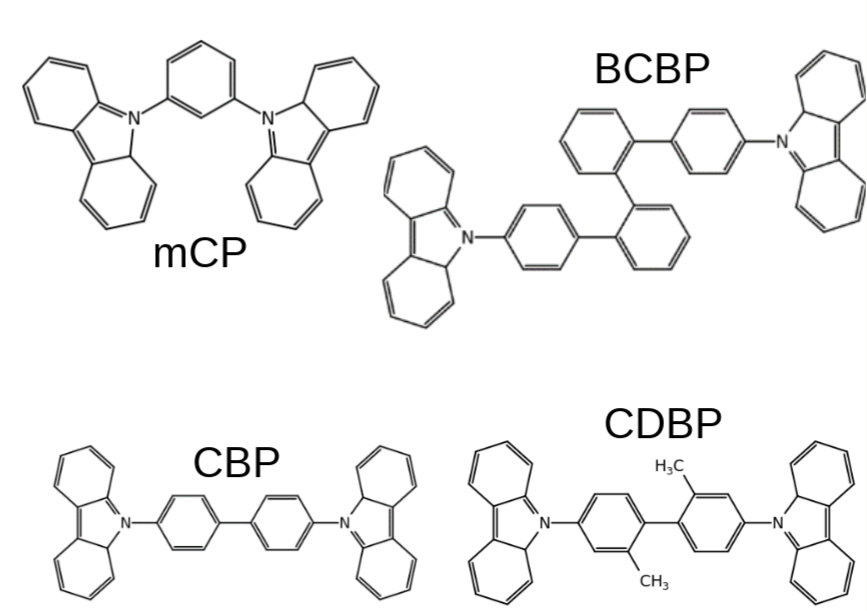
\includegraphics[width=.5\textwidth]{hosts/molecules}
\caption{Host molecules used in this study.}
\label{fig:hosts_molecules}
\end{wrapfigure}

Design rules for understanding the degradation behavior of OLED materials are not well understood.
It can be difficult to isolate molecular property differences in devices, when changes in a molecule can affect many different device parameters, such as energy levels, mobilities, morphology, and the optical properties.
It is therefore imperative to investigate closely related molecules and examine the affects on device performance.
This provides the most isolation of device parameters and allows the most fundamental study of stability of the molecules.
One of the most widely studies host molecule families is the carbazoles, with 4,4'-Bis(N-carbazolyl)-1,1'-biphenyl (CB) and 1,3-Bis(N-carbazolyl)benzene (mCP) being extremely popular hosts for green and blue devices, respectively.
A series of closely related molecules is also readily available, including 2,2'-Bis(4-(carbazol-9-yl)phenyl)-biphenyl (BCBP) and 4,4'-Bis(9-carbazolyl)-2,2'-dimethylbiphenyl (CDBP).
These molecules, all shown in Figure \ref{fig:hosts_molecules} provide a testing ground for investigating a molecular host family in a device system.
This chapter seeks to compare the behavior of devices utilizing these hosts and understand their relative behavior from a molecular level.


\section{Electrical Characterization}

\begin{figure}[ht]
\centering
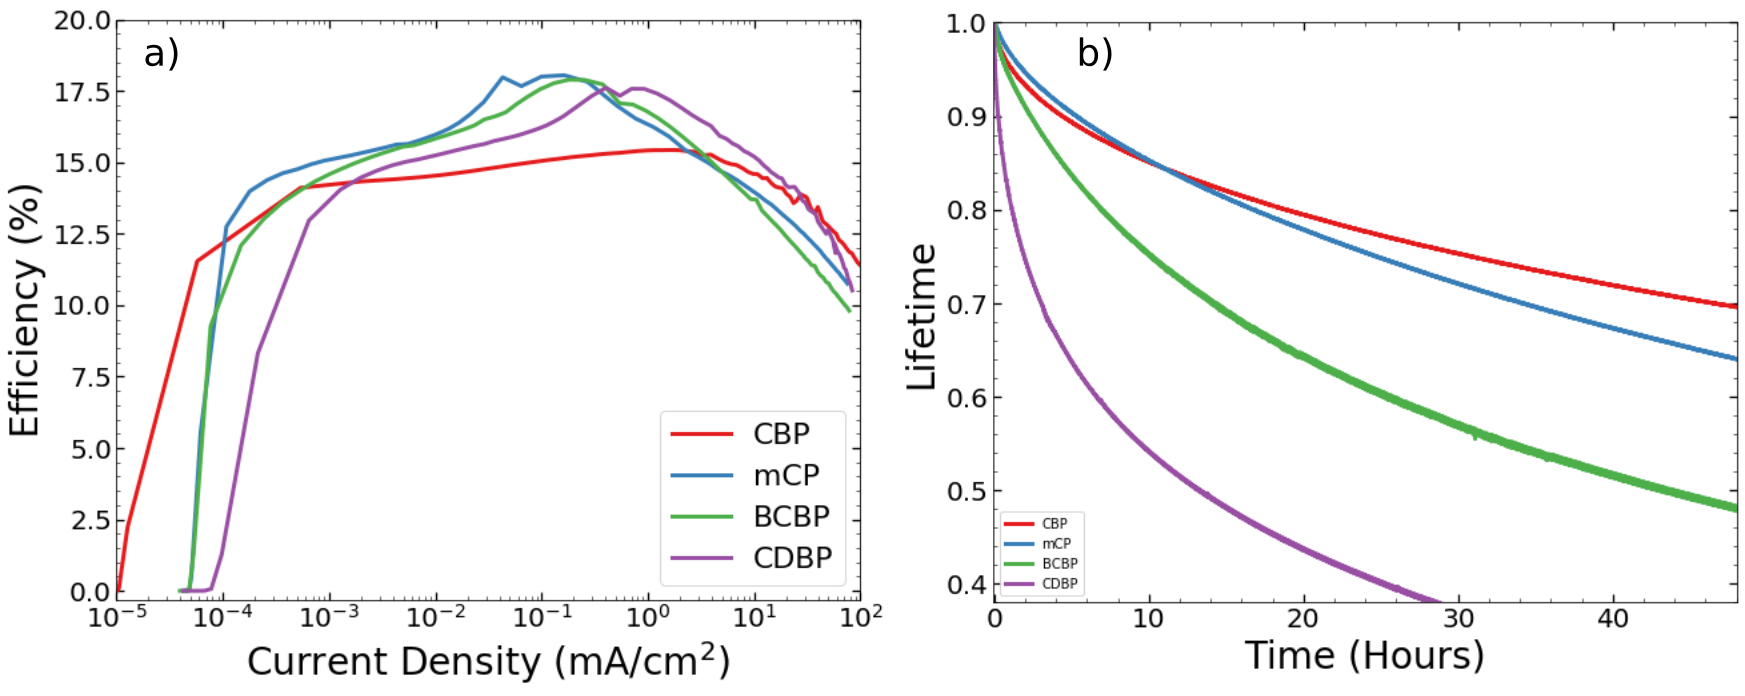
\includegraphics[width=.8\textwidth]{hosts/el}
\caption{(a) External quantum efficiency \eqe for all hosts.  Similar peak \eqe is seen. (b) EL lifetime for all hosts.}
\label{fig:hosts_el}
\end{figure}

Devices were prepared consisting of an ITO patterned substrate followed by 40 nm of TCTA.
The EML of all devices was 20 nm thick with the host doped with 5\% \irppy.
A 40 nm thick TPBi ETL with an LiF/Al cathode finished off the devices.

Device \eqe can be seen in Figure \ref{fig:hosts_el}a, as was similar between all devices.  
All devices showed a slow rise in efficiency, peaked between $10^{-1}-10^0$ mA/cm$^2$.
The electrical lifetimes were characterized for these devices at 1000 cd/m$^2$, and are shown in Figure \ref{fig:hosts_el}b.
Here, CBP shows the peak lifetime, though is comparable to mCP.
BCBP shows a significant reduction in lifetime, with CDBP being the lowest performing device.


\begin{figure}[ht]
\centering
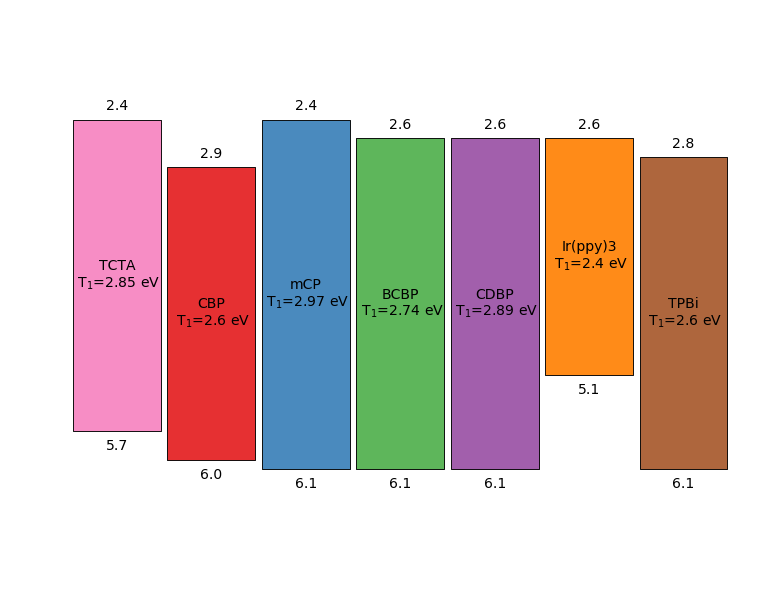
\includegraphics[width=.5\textwidth]{hosts/energy}
\caption{Energy levels for all materials used in devices.  Triplet energies for the hosts are measured by low temperature phosphorescence, described in Appendix \ref{sec:triplets}.}
\label{fig:hosts_energy}
\end{figure}

Energy levels for all of these materials are shown in Figure \ref{fig:hosts_energy}.
Triplet energies are extracted from low temperature phosphorescence, discussed in Appendix \ref{sec:triplets}.

From the EL lifetimes, there is no apparent trend with obvious device parameters, such as efficiency or driving voltage, or with semiconductor properties such as energy levels or triplet energies.
This lack of dependence can be seen in Figure \ref{fig:hosts_trends}.
Without a clear explanation for this trend from the bulk and device properties, this suggests an explanation for device stability from a more fundamental level, possibly intrinsic to the molecule.

\begin{figure}[ht]
\centering
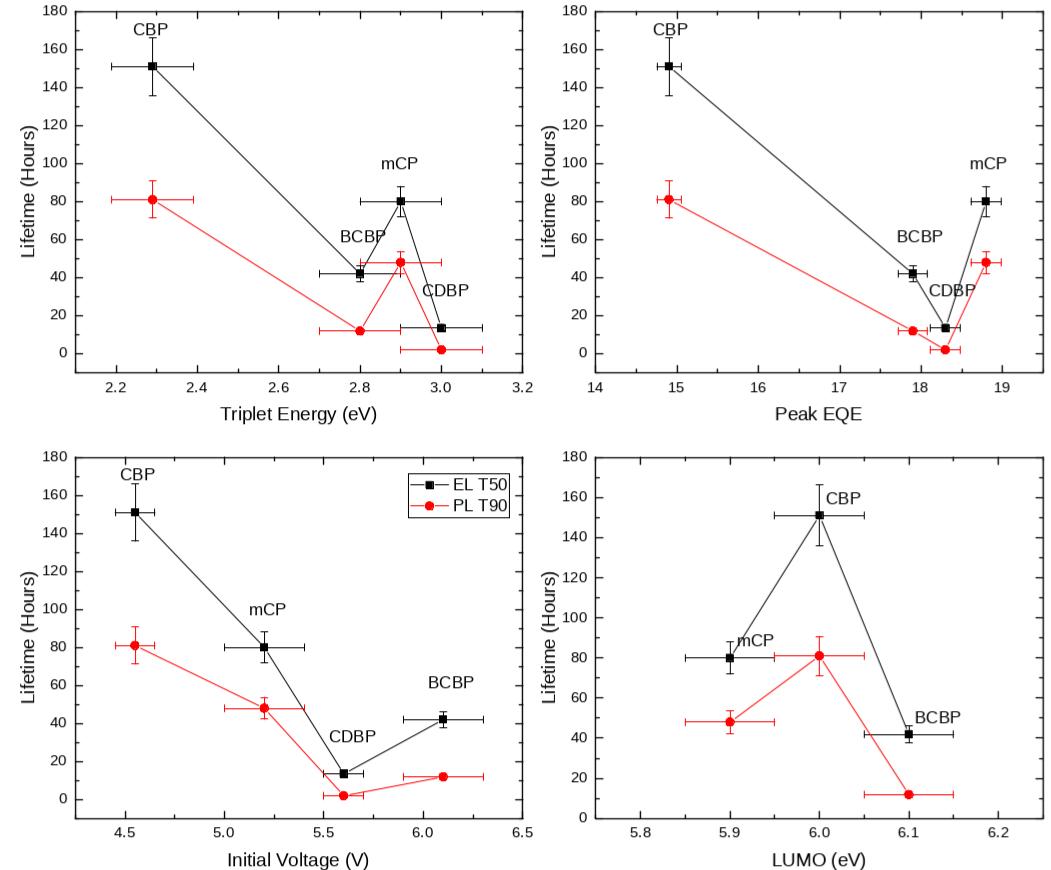
\includegraphics[width=.5\textwidth]{hosts/trends}
\caption{}
\label{fig:hosts_trends}
\end{figure}


\section{Optical Characterization}

Without an explanation for the electrical behavior, degradation behavior of the hosts was sought outside of a device and in the absence of electrical pumping.
Therefore, photostability was investigated.
Section \ref{sec:hosts_spectral} goes into detail about the optical characterization of the hosts and the development of the optical degradation technique, while Section \ref{sec:hosts_stability} talks about the performance of these hosts.


\subsection{Spectral Characterization}\label{sec:hosts_spectral}


\begin{wrapfigure}{r}{.5\textwidth}
\centering
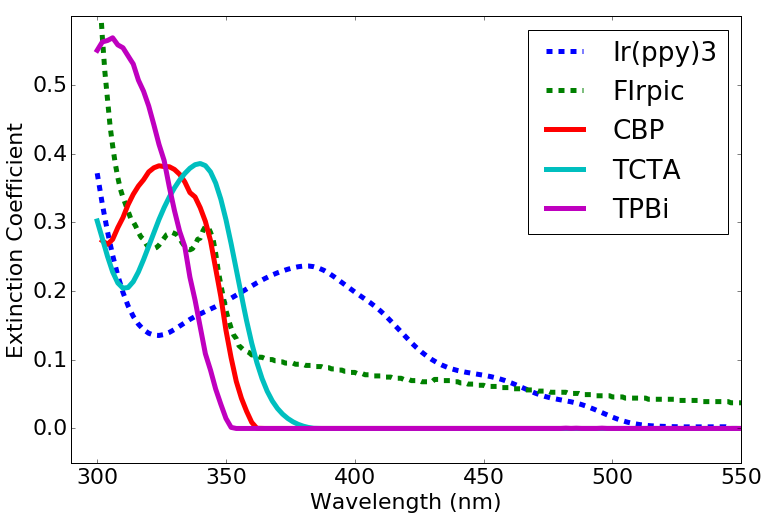
\includegraphics[width=.5\textwidth]{hosts/optical_k}
\caption{Optical constant $k$ for all hosts turn on between 340-350 nm. }
\label{fig:hosts_k}
\end{wrapfigure}

When doing optical degradation, the intensity of the emitter PL is observed as a function of time.
There are two pumping schemes that we want to consider here: pumping the host with transfer to the emitter, or pumping the emitter directly.
These two schemes offer different unique dynamics with regard to the degradation behavior.

When pumping the host, exciton formation occurs on the hosts, allowing stress on the host molecule, and potential for high energy bimolecular events.
The transfer event of the exciton to the emitter molecule will have a rate, $k_T$ that may be competitive with non-radiative decay on the host, $k_{nr}$.  
The efficiency of this transfer even can be expressed as 

\begin{equation}
\eta_T=\frac{k_T}{k_T +k_{nr}}.
\end{equation}

When pumping the host during degradation, any loss in $\eta_T$ during degradation will be convoluted with PL loss from the emitter, \pl.
In addition to the stress on the host, the energy transfer of the exciton from the host to the guest is exothermic, due to the lower triplet energy of the guest.
This results in additional heat being dumped into the system, with the potential to accelerate degradation.
Another issue is that the guest molecule can still absorb directly, so may be convoluted into the interpretation of this data.
It should be noted that based on the absorption strength weighted to molecular density, shown in Figure \ref{fig:hosts_k}, \irppy is still absorbing, though most absorption events below 350 nm will be on the host.

Alternatively, the guest may be pumped directly, by pumping above the absorption band edge of the host, which for these molecules is between 340-350 nm, as shown in Figure \ref{fig:hosts_k}.
This is a simpler measurement and provides a more direct measurement of the stability of excitons on the guest molecule decaying.
Which technique is more representative of the behavior in devices could be debated depending on the exciton formation mechanism within the device, and if excitons are formed on the host during EL.
Given the low HOMO level of  \irppy relative to the hosts, it is likely that \irppy serves as a hole trap in devices and is responsible for some of the hole transport, and is unlikely that excitons form on the host.

\begin{figure}[ht]
\centering
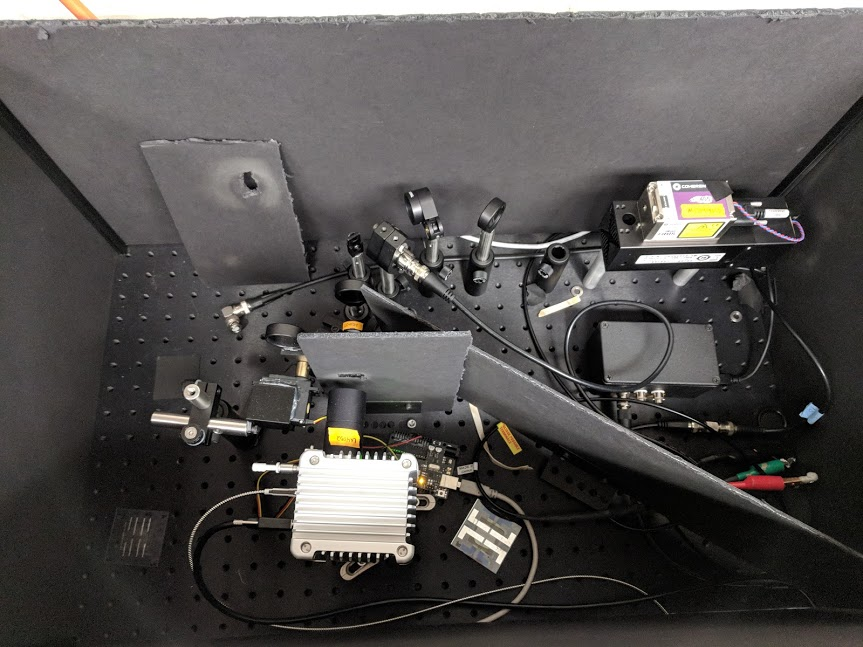
\includegraphics[width=.6\textwidth]{hosts/setup}
\caption{PL degradation setup. Silver box in the bottom is the LDLS, and has attached lens tube containing collimation lenses.  This is followed by a primitive cardboard iris, then a servo motor controlled mechanical shutter.  This is followed by a wavelength filter, before reaching the sample mount in the top left, with collection diode at a 45$\degree$ angle.  The laser beam path follows the top of the box, with the laser on the top right.}
\label{fig:hosts_setup}
\end{figure}

To optically degrade devices, the setup shown in Figure \ref{fig:hosts_setup} has been developed.
This box features a 405 nm laser, as well as a white light source (LDLS, Energetiq) for pumping PL of devices, and can measure PL intensity of the device during degradation.
The LDLS is a relatively flat spectral white light source, and can be filtered to provide pumping at various wavelength ranges.

\begin{wrapfigure}{r}{.5\textwidth}
\centering
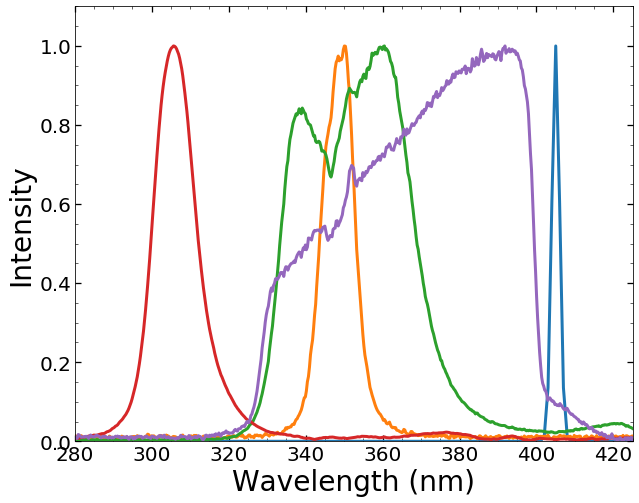
\includegraphics[width=.5\textwidth]{hosts/spectra}
\caption{Available lamp spectra for photo degradation. Blue is the 405 nm laser, green is a 350 nm bandpass with 40 nm FWHM, yellow is a 350 nm bandpass with a 10 nm FWHM, purple is a 325 long pass in combination with a 400 nm shortpass, and red is a 300 nm bandpass with 10 nm FWHM. }
\label{fig:hosts_spectra}
\end{wrapfigure}

Filtered pump spectra relevant to this study are shown in Figure \ref{fig:hosts_spectra}.
This provides a variety of pumping schemes for this study, but all data presented will use either the 405 nm laser, or the 350 nm 40 nm FWHM filter, shown in Figure \ref{fig:hosts_spectra} in blue and green, respectively.
The 350 nm and 405 nm pumps allow excitation of the host and guest, respectively.
In addition to single wavelength degradation, the relative loss in $\eta_T$ can be assessed by pumping with 350 nm light with a low duty cycle excitation from the 405 nm light to probe the guest directly.
This is implemented by temporarily shuttering the LDLS lamp using a servo motor shutter.
The 405 nm laser can be turned on and off with reliable power quickly, as previously shown in Chapter \ref{sec:integrated_lifetime}.
Using this method, problems with the host energy transfer can be separated from the guest stability.


\subsection{Photostability}\label{sec:hosts_stability}


For preliminary investigation into the optical stability of these hosts, the 350 nm lamp was used with an intermittent probe from the 405 nm laser.
Films for this degradation consisted of the full device stack including cathode, but excluding the planarizing layer at the ITO (AQ1250) and excluding LiF at the cathode.
LiF has been shown to dissociate under strong optical excitation.\supercite{Wang2011a}
The full stack with cathode was used because rapid degradation was seen even when encapsulated without the cathode, hinting at oxygen quenching of the film.
At 350 nm, TCTA is being excited as well as the host, but shows much a bluer emission spectra, and is filtered from the collected signal by a 450 nm long pass filter on the detector.


Host stability can be seen in Figure \ref{fig:hosts_pl350_405} with the 350 nm and 405 nm signal shown in (a) and (b) respectively.
This optical degradation shows the same trend with host as the electrical degradation, further evidencing that the stability in devices is due to the intrinsic stability of the host material, rather than an effect of the manufactured device.
The signal at 405 nm also follows the same trend, but with much less degradation than the 350 nm pump.
This suggests that the majority of the degradation seen is in $\eta_T$ or in the host absorption.

\begin{wrapfigure}{r}{.5\textwidth}
\centering
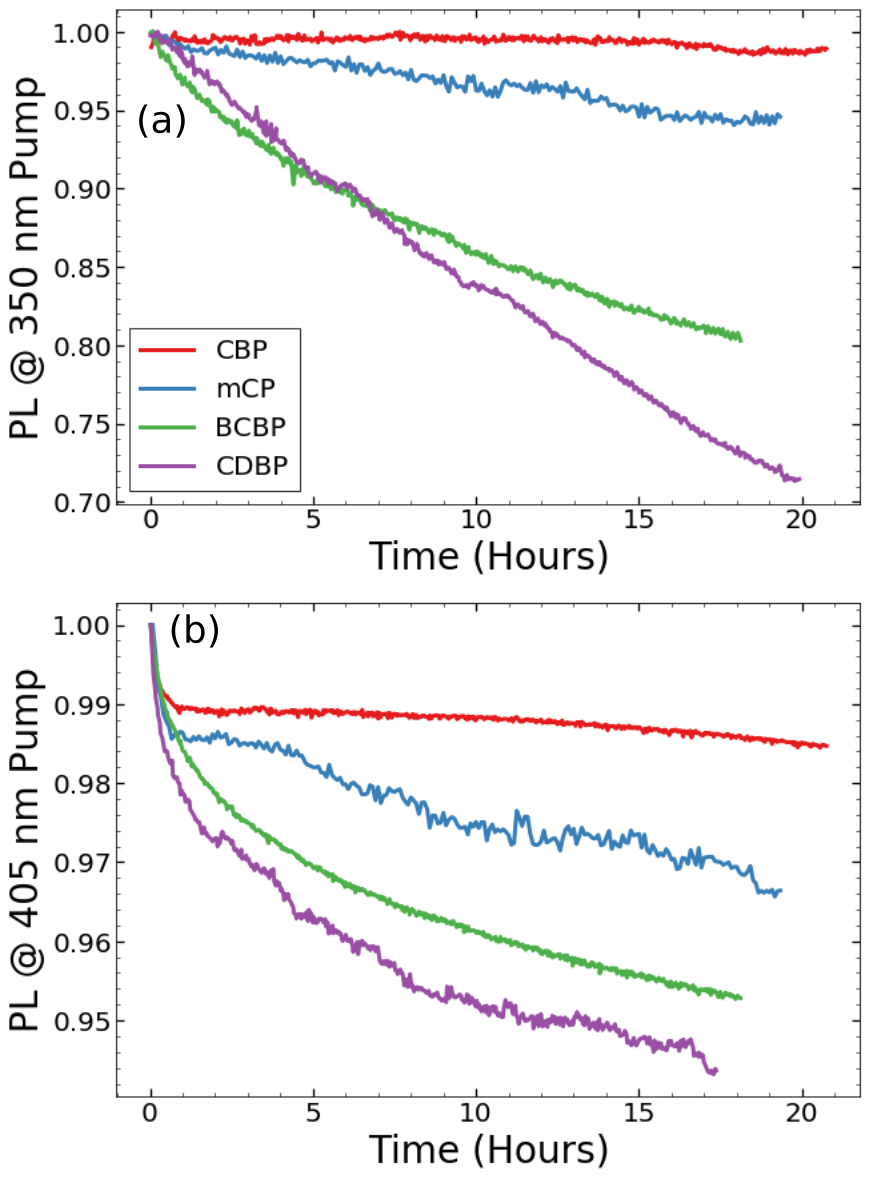
\includegraphics[width=.5\textwidth]{hosts/pl_lifetimes_350_405}
\caption{Photodegradation at 350 nm, with intermittent probe at 405 nm. }
\label{fig:hosts_pl350_405}
\end{wrapfigure}

With these results, it was hypothesized that the degradation in the 350 nm signal was due to loss in $\eta_T$ and degradation of the host.
The loss in 405 nm signal could be due to quenching of \irppy by the degradation products of the host molecule.
Under this assumption, if the host is not pumped, identical behavior between the four devices would be observed.


Therefore, the same devices were degraded under a 405 nm pump only, as shown in Figure \ref{fig:hosts_pl405}.
Contrary to the hypothesis, the behavior differed between hosts, rather than being identical.
This is interesting because if the host is not being excited, this would suggest that simply the environment around the guest exciton on neighboring molecules is accelerating degradation.
This could be due to a morphological effect, or a change in non-radiative pathways of the guest exciton.  

\begin{wrapfigure}{r}{.5\textwidth}
\centering
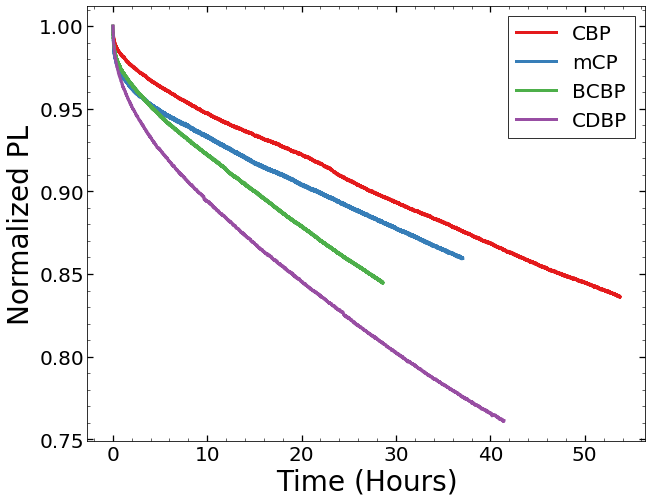
\includegraphics[width=.5\textwidth]{hosts/pl_lifetimes_405}
\caption{Photodegradation at 405 nm. }
\label{fig:hosts_pl405}
\end{wrapfigure}

Alternatively, it is possible that under high exciton density, bimolecular quenching is transferring excitons onto the host.
Though these excitons would be short lived when compared to the guest excitons, they would be high energy and relax quickly, similar to bimolecular degradation mechanisms suggested for EL lifetimes.\supercite{Giebink2008a,Bangsund2018}
This situation is difficult to avoid absolutely.
While going to lower emitter concentration to try to spatially separate the emitter and pumping at lower flux may increase the exciton spacing on average, high exciton density regions would still exist and it is plausible that the observed degradation is caused by these rare, but still active pathways.
Additionally, if any sort of aggregation is observed with the emitter, and has been observed for some devices, then bimolecular quenching is always possible, regardless of doping concentration.\supercite{Reineke2009}

Despite these hesitations, if low doping concentration does show the same decay behavior, this would indicate host excitons.
Devices were tested with 1\% \irppy, shown in Figure \ref{fig:hosts_pl405_1pct}.
Interestingly, a difference is still observed, but CDBP and BCBP trade places.

\begin{figure}[ht]
\centering
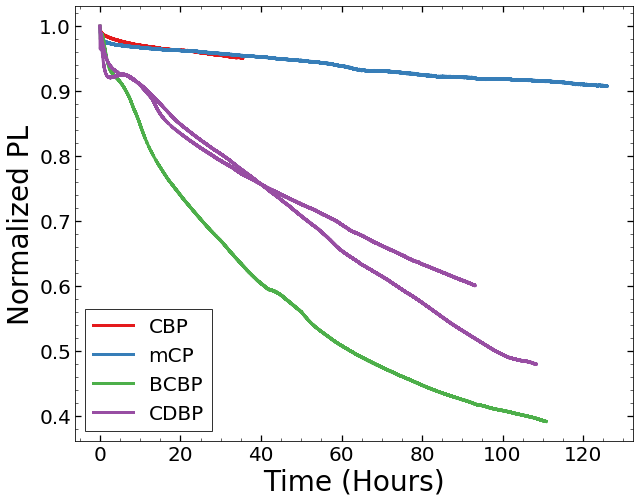
\includegraphics[width=.5\textwidth]{hosts/pl_lifetimes_405_1pct}
\caption{Photodegradation at 405 nm. }
\label{fig:hosts_pl405_1pct}
\end{figure}

\section{Ongoing Research}


The working hypothesis for these devices is still that host excitons are being formed through bimolecular processes.
To prove this hypothesis, it must be shown that guest excitons are still being excited.
This could be done through an excited state absorption measurement.\supercite{Laming1988,Ichimura1987}
Excitons on the host would have a separate signature than excitons on the guest.
While emission is not seen from host excitons because they transfer to the guest, the host excitons would still have absorption.
One problem with this technique is that the host exciton population would be very low when compared with the excited guest, and the host exciton absorption could be lost in the noise.

An alternative explanation for the observed behavior is morphological differences with regards to the \irppy molecules.
\irppy has been previously shown to aggregate in dilute thin films.\supercite{Reineke2009}
If differences in the aggregation of \irppy occur between the hosts, this could influence the degradation.
To investigate this, \pl is being investigated as a function of concentration and host to see if differences in aggregation are observed.
For more aggregated \irppy, one would expect a lower \pl, and possible a change in the relative \pl with doping concentration between hosts due to a critical doping concentration to enable aggregation.
Great care must be taken in the doping concentrations of these measurements to ensure that observed differences in \pl are due to differences between the hosts, and not error in the doping concentration.
If a difference in \pl is observed, then TEM imaging will be used to see clusters of Iridium in the films.
We expect that larger clusters would correspond to lower \pl, and may correlate with the observed trend in lifetime.

\ifcsdef{mainfile}{}{\printbibliography}
\end{document}
